\documentclass[11pt]{article}

\usepackage[letterpaper,margin=0.72in]{geometry}
\usepackage[T1]{fontenc}
\usepackage{lmodern}
\usepackage{microtype}
\usepackage{amsmath,amssymb}
\usepackage{booktabs}
\usepackage{enumitem}
\usepackage{xcolor}
\usepackage{tikz}
\usetikzlibrary{arrows.meta,calc,positioning}
\usepackage[colorlinks=true,linkcolor=blue!55!black,urlcolor=blue!55!black]{hyperref}
\usepackage{fancyhdr}

\definecolor{navy}{HTML}{163A5F}
\definecolor{blueaccent}{HTML}{2474A6}
\definecolor{orangeaccent}{HTML}{D97706}
\definecolor{softblue}{HTML}{EAF3F8}
\definecolor{softorange}{HTML}{FFF3E3}
\definecolor{darkgray}{HTML}{38434F}

\pagestyle{fancy}
\fancyhf{}
\lhead{\textcolor{navy}{\small Torque-Spool Demonstration}}
\rhead{\textcolor{darkgray}{\small Physics Walkthrough}}
\cfoot{\textcolor{darkgray}{\thepage}}
\renewcommand{\headrulewidth}{0.4pt}
\setlength{\headheight}{14pt}
\setlength{\parindent}{0pt}
\setlength{\parskip}{5pt}
\setlist[itemize]{leftmargin=1.35em,itemsep=2pt,topsep=3pt}
\setlist[enumerate]{leftmargin=1.55em,itemsep=3pt,topsep=3pt}

\newcommand{\keybox}[1]{%
  \begin{center}
  \fcolorbox{blueaccent}{softblue}{%
    \begin{minipage}{0.88\linewidth}
    \centering\vspace{3pt}#1\vspace{3pt}
    \end{minipage}}
  \end{center}}

\newcommand{\notebox}[1]{%
  \begin{center}
  \fcolorbox{orangeaccent}{softorange}{%
    \begin{minipage}{0.88\linewidth}
    \vspace{3pt}#1\vspace{3pt}
    \end{minipage}}
  \end{center}}

\newcommand{\manualheader}{%
  \thispagestyle{plain}%
  \noindent\textcolor{navy}{\small Torque-Spool Demonstration}%
  \hfill\textcolor{darkgray}{\small Physics Walkthrough}\par
  \vspace{2pt}\hrule\vspace{12pt}}

\begin{document}

\begin{center}
  {\color{navy}\LARGE\bfseries Why Does the Spool Reverse Direction?}\par
  \vspace{3pt}
  {\large A Newton-Euler walkthrough for the spool-paradox demonstration}\par
  \vspace{5pt}
  {\color{darkgray}\small Tire-on outer diameter: $D=185.0\,\mathrm{mm}$ \quad | \quad rolling radius: $R=92.5\,\mathrm{mm}$}
\end{center}

\section*{1. System, forces, and sign conventions}

A cord is tangent to an inner winding cylinder of radius $r$ while the spool rolls on outer tires of radius $R$. The cord is pulled with tension $T$ at angle $\theta$ above the horizontal. The direction of the spool's acceleration changes at a critical angle $\theta_{\mathrm c}$.

Take $+x$ to the right, positive angular acceleration $\alpha$ counterclockwise, and let the static-friction force $f$ be signed. The leftward friction arrow below is the direction obtained for the usual geometry; the equations themselves determine its sign.

\begin{center}
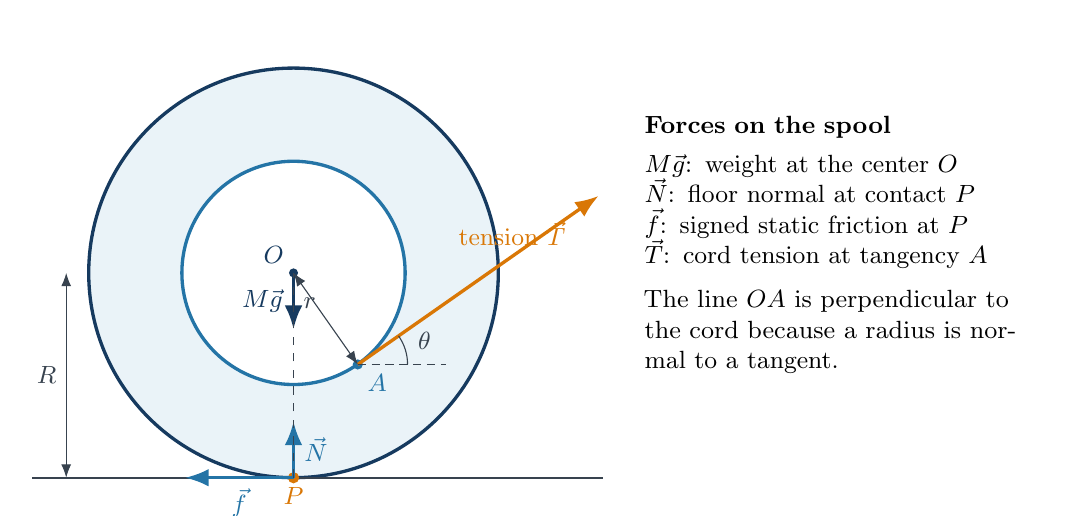
\begin{tikzpicture}[scale=1.02,>=Latex,font=\small]
  \coordinate (O) at (0,0);
  \coordinate (P) at (0,-2.55);
  \coordinate (A) at (0.80,-1.14);

  \fill[softblue] (O) circle (2.55);
  \draw[navy,very thick] (O) circle (2.55);
  \fill[white] (O) circle (1.39);
  \draw[blueaccent,very thick] (O) circle (1.39);
  \draw[darkgray,thick] (-3.25,-2.55)--(3.85,-2.55);
  \fill[navy] (O) circle (1.6pt) node[above left] {$O$};
  \fill[orangeaccent] (P) circle (2pt) node[below] {$P$};
  \fill[blueaccent] (A) circle (1.8pt) node[below right] {$A$};

  % Every force vector begins at its physical point of application.
  \draw[orangeaccent,very thick,-{Latex[length=3mm]}] (A)--++(3.0,2.10)
    node[pos=0.64,above] {tension $\vec T$};
  \draw[navy,very thick,-{Latex[length=3mm]}] (O)--++(0,-0.70)
    node[midway,left] {$M\vec g$};
  \draw[blueaccent,very thick,-{Latex[length=3mm]}] (P)--++(0,0.70)
    node[midway,right] {$\vec N$};
  \draw[blueaccent,very thick,-{Latex[length=3mm]}] (P)--++(-1.35,0)
    node[midway,below] {$\vec f$};

  \draw[<->,darkgray] (-2.83,0)--(-2.83,-2.55)
    node[midway,left] {$R$};
  \draw[<->,darkgray] (O)--(A)
    node[midway,above left] {$r$};
  \draw[darkgray,dashed] (P)--(O);
  \draw[darkgray,densely dashed] (A)--++(1.10,0);
  \draw[darkgray] ($(A)+(0.62,0)$) arc[start angle=0,end angle=35,radius=0.62];
  \node[darkgray] at ($(A)+(0.83,0.30)$) {$\theta$};

  \node[align=left,text width=5.0cm,anchor=west] at (4.25,0.35) {
    \textbf{Forces on the spool}\\[3pt]
    $M\vec g$: weight at the center $O$\\
    $\vec N$: floor normal at contact $P$\\
    $\vec f$: signed static friction at $P$\\
    $\vec T$: cord tension at tangency $A$\\[5pt]
    The line $OA$ is perpendicular to the cord because a radius is normal to a tangent.
  };
\end{tikzpicture}
\end{center}

\keybox{\textbf{Rolling constraint:} with the signs chosen above, rolling without slipping requires
\[
a=-R\alpha.
\]}

\newpage
\manualheader
\section*{2. Newton's laws and the rolling acceleration}

Let $M$ be the total spool mass and $I$ its moment of inertia about $O$. Newton's second law in the horizontal and vertical directions gives
\begin{align}
  \sum F_x &: \qquad T\cos\theta+f=Ma, \label{eq:fx}\\
  \sum F_y &: \qquad N+T\sin\theta-Mg=0. \label{eq:fy}
\end{align}
The vertical acceleration is zero while the spool stays on the floor, so
\begin{equation}
  N=Mg-T\sin\theta. \label{eq:normal}
\end{equation}

Now sum torques about the center $O$. The tension is tangent to radius $r$, and friction acts with lever arm $R$. With counterclockwise torque positive,
\begin{equation}
  \sum\tau_O=rT+Rf=I\alpha. \label{eq:torque}
\end{equation}
Use the rolling condition $\alpha=-a/R$ and solve Eq.~\eqref{eq:fx} for $f$:
\[
  f=Ma-T\cos\theta.
\]
Substitution into Eq.~\eqref{eq:torque} gives
\begin{align*}
  rT+R\left(Ma-T\cos\theta\right)&=-\frac{I}{R}a,\\
  T\left(r-R\cos\theta\right)
  +a\left(MR+\frac{I}{R}\right)&=0.
\end{align*}

Define two dimensionless quantities,
\[
  \rho=\frac{r}{R},
  \qquad
  \kappa=\frac{I}{MR^2}.
\]
The acceleration and the signed friction force are then
\begin{align}
  \boxed{\displaystyle
  a=\frac{T}{M}\,
  \frac{\cos\theta-\rho}{1+\kappa}}
  \label{eq:accel}\\[4pt]
  \boxed{\displaystyle
  f=-T\,
  \frac{\rho+\kappa\cos\theta}{1+\kappa}.}
  \label{eq:friction}
\end{align}

Equation~\eqref{eq:accel} contains the reversal directly. Because $T/M$ and $1+\kappa$ are positive, only $\cos\theta-\rho$ determines the sign of $a$:
\begin{center}
\begin{tabular}{@{}lll@{}}
\toprule
Condition & Sign of $a$ & Motion from rest\\
\midrule
$\cos\theta>\rho$ & $a>0$ & accelerates toward $+x$\\
$\cos\theta=\rho$ & $a=0$ & transition point\\
$\cos\theta<\rho$ & $a<0$ & accelerates toward $-x$\\
\bottomrule
\end{tabular}
\end{center}

\keybox{\LARGE $\displaystyle
a=0
\quad\Longrightarrow\quad
\cos\theta_{\mathrm c}=\frac{r}{R}
\quad\Longrightarrow\quad
\theta_{\mathrm c}=\cos^{-1}\left(\frac{r}{R}\right).$}

\newpage
\section*{3. Geometry of the critical angle}

The same result has a useful geometric interpretation. At the transition, extend the cord's line of action backward from the tangency point $A$. It passes through the floor-contact point $P$. The tension vector itself still begins at $A$, its physical point of application.

\begin{center}
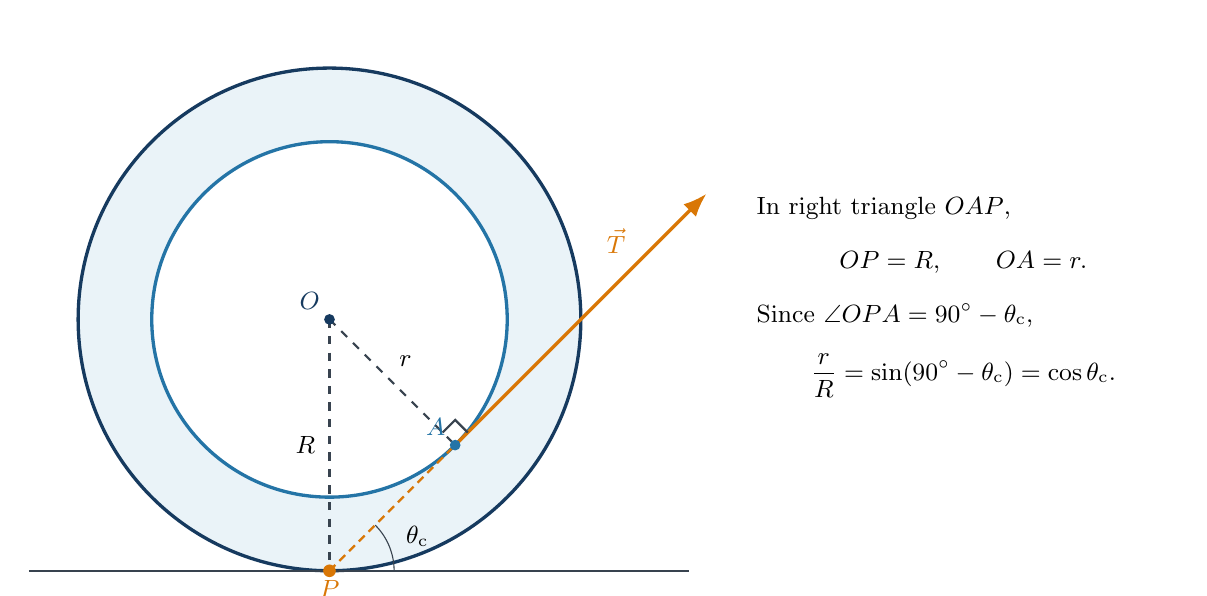
\begin{tikzpicture}[scale=1.14,>=Latex,font=\small]
  \coordinate (O) at (0,0);
  \coordinate (P) at (0,-2.8);
  \coordinate (A) at (1.4,-1.4);

  \fill[softblue] (O) circle (2.8);
  \draw[navy,very thick] (O) circle (2.8);
  \fill[white] (O) circle (1.98);
  \draw[blueaccent,very thick] (O) circle (1.98);
  \draw[darkgray,thick] (-3.35,-2.8)--(4.0,-2.8);
  \draw[orangeaccent,densely dashed,thick] (P)--(A);
  \draw[orangeaccent,very thick,-{Latex[length=3mm]}] (A)--(4.2,1.4)
    node[pos=0.72,above left] {$\vec T$};
  \draw[darkgray,dashed,thick] (O)--(A);
  \draw[darkgray,dashed,thick] (O)--(P);
  \fill[navy] (O) circle (1.7pt) node[above left] {$O$};
  \fill[orangeaccent] (P) circle (2pt) node[below] {$P$};
  \fill[blueaccent] (A) circle (1.7pt) node[above left] {$A$};

  \node[left] at (-0.05,-1.4) {$R$};
  \node[above right] at (0.67,-0.63) {$r$};
  \draw[darkgray] ($(P)+(0.72,0)$) arc[start angle=0,end angle=45,radius=0.72];
  \node at ($(P)+(0.98,0.38)$) {$\theta_{\mathrm c}$};
  \draw[darkgray,thick] ($(A)+(-0.14,0.14)$)--($(A)+(0,0.28)$)--($(A)+(0.14,0.14)$);

  \node[align=left,text width=5.25cm,anchor=west] at (4.65,0.25) {
    In right triangle $OAP$,
    \[
      OP=R,\qquad OA=r.
    \]
    Since $\angle OPA=90^\circ-\theta_{\mathrm c}$,
    \[
      \frac{r}{R}
      =\sin(90^\circ-\theta_{\mathrm c})
      =\cos\theta_{\mathrm c}.
    \]
  };
\end{tikzpicture}
\end{center}

\keybox{\LARGE $\displaystyle
\theta_{\mathrm c}
=\cos^{-1}\left(\frac{r}{R}\right)
=\cos^{-1}\left(\frac{2r}{D}\right).$}

\section*{4. Numerical check for the 45-degree insert}

For the installed TPU tires,
\[
  D=185.0\,\mathrm{mm},
  \qquad
  R=\frac{D}{2}=92.5\,\mathrm{mm}.
\]
The 45-degree insert has $r=65.407\,\mathrm{mm}$, so
\[
\begin{aligned}
  \theta_{\mathrm c}
  &=\cos^{-1}\left(\frac{65.407\,\mathrm{mm}}{92.5\,\mathrm{mm}}\right)\\
  &=45.00^\circ.
\end{aligned}
\]

For cord diameter $d$, the first-layer centerline radius is
\[
  r_{\mathrm{eff}}=r+\frac{d}{2}.
\]
A $2.0\,\mathrm{mm}$ cord gives $r_{\mathrm{eff}}=66.407\,\mathrm{mm}$ and
$\theta_{\mathrm c,eff}\approx44.12^\circ$.

\newpage
\manualheader
\section*{5. Static-friction condition for no slipping}

\notebox{\textbf{Terminology.} The relevant material property is the coefficient of \emph{static friction} $\mu_s$. The coefficient of restitution $e$ describes energy retained in an impact or bounce and does not set the rolling-slip threshold in this slow demonstration.}

Coulomb static friction requires
\begin{equation}
  |f|\leq\mu_s N. \label{eq:noslip}
\end{equation}
Using Eqs.~\eqref{eq:normal} and \eqref{eq:friction}, the general required coefficient is
\begin{equation}
  \boxed{\displaystyle
  \mu_{\mathrm{req}}(\theta)
  =
  \frac{T\left|\rho+\kappa\cos\theta\right|}
  {(1+\kappa)\left(Mg-T\sin\theta\right)}.}
  \label{eq:mureqgeneral}
\end{equation}
This formula applies while $N>0$, or equivalently $T\sin\theta<Mg$.

At the critical angle, $\rho=\cos\theta_{\mathrm c}$. The dependence on the moment of inertia cancels:
\[
  |f_{\mathrm c}|=T\cos\theta_{\mathrm c},
  \qquad
  N_{\mathrm c}=Mg-T\sin\theta_{\mathrm c}.
\]
Let the dimensionless pull be $q=T/(Mg)$. The critical-angle slip test becomes
\begin{align}
  \boxed{\displaystyle
  \mu_{\mathrm{req,c}}
  =\frac{q\cos\theta_{\mathrm c}}
  {1-q\sin\theta_{\mathrm c}}}
  \label{eq:mucritical}\\[4pt]
  \boxed{\displaystyle
  q\leq q_{\max}
  =\frac{\mu_s}
  {\cos\theta_{\mathrm c}+\mu_s\sin\theta_{\mathrm c}}.}
  \label{eq:qmax}
\end{align}

\subsection*{How much do the larger angles matter?}

The table uses a representative pull $q=0.20$, meaning $T=0.20Mg$. It is a dimensionless illustration, not a measurement of the apparatus.

\begin{center}
\begin{tabular}{@{}rrrr@{}}
\toprule
$\theta_{\mathrm c}$ &
$N_{\mathrm c}/(Mg)$ &
$|f_{\mathrm c}|/(Mg)$ &
$\mu_{\mathrm{req,c}}$\\
\midrule
$30^\circ$ & 0.900 & 0.173 & 0.192\\
$40^\circ$ & 0.871 & 0.153 & 0.176\\
$45^\circ$ & 0.859 & 0.141 & 0.165\\
$50^\circ$ & 0.847 & 0.129 & 0.152\\
$60^\circ$ & 0.827 & 0.100 & 0.121\\
\bottomrule
\end{tabular}
\end{center}

From $30^\circ$ to $60^\circ$, the normal force falls only from $0.900Mg$ to $0.827Mg$ (about an 8\% change). Meanwhile, the horizontal tension that friction must balance falls more strongly. The required friction coefficient therefore \emph{decreases}, from about 0.192 to 0.121 in this example. Larger critical angles slightly unload the tire, but they do not make slip more likely here; the friction margin improves.

\keybox{For any planned pull, compute $q=T/(Mg)$ and compare Eq.~\eqref{eq:mucritical} with the available $\mu_s$, or use Eq.~\eqref{eq:qmax} to find the largest no-slip pull.}

\newpage
\section*{6. Suggested classroom procedure}

\begin{enumerate}
  \item Install the desired insert and both TPU tires. Use a thin cord in one neat layer.
  \item Measure the spool mass $M$ and, if quantitative testing is desired, measure the pull $T$ with a spring scale or force sensor.
  \item Pull slowly at an angle clearly below the label and note the acceleration direction.
  \item Repeat clearly above the label and observe the reversal.
  \item Approach the transition in small angular steps. Compare the result with
  \[
    \theta_{\mathrm c}
    =\cos^{-1}\left(\frac{r}{R}\right),
  \]
  or replace $r$ by $r+d/2$ when correcting for cord thickness.
  \item Evaluate the no-slip margin using
  \[
    q=\frac{T}{Mg},
    \qquad
    \mu_{\mathrm{req,c}}
    =\frac{q\cos\theta_{\mathrm c}}
    {1-q\sin\theta_{\mathrm c}}.
  \]
  \item Discuss why taking torques about the floor-contact point gives the same critical-angle condition: the normal force, friction, and weight all have zero moment about that point at the transition, and the tension line passes through it.
\end{enumerate}

\section*{7. Model assumptions and interpretation}

\begin{itemize}
  \item The spool is rigid, the floor is level, and the cord stays taut and tangent to the winding cylinder.
  \item The no-slip derivation uses static friction and the rolling constraint $a=-R\alpha$.
  \item The cord is treated as massless. Additional winding layers increase the effective radius and lower the critical angle.
  \item Axle losses, rolling resistance, tire deformation, and three-dimensional misalignment are neglected.
  \item The sign of the acceleration predicts the initial rolling direction. Exactly at the ideal transition, the tension produces no rolling acceleration; small losses and imperfections can dominate.
\end{itemize}

\keybox{\textbf{Central result:} Newton's laws, the rolling constraint, and the tangent geometry all lead to
\[
\theta_{\mathrm c}=\cos^{-1}\left(\frac{r}{R}\right).
\]
The static-friction test is separate: it checks whether the assumed rolling motion can occur without slipping.}

\vfill
\begin{center}
\small\color{darkgray}
Dimensions correspond to the supplied spool with both TPU tires installed.
\end{center}

\end{document}
